\subsection{Potencial Lennard-Jones}

A nivel microscópico las interacciones entre moléculas pueden describirse de manera aproximada por medio del potencial de Lennard-Jones:

\begin{equation}
	V(r) = 4\epsilon \left( \left( \frac{\sigma}{r} \right) ^{12} - \left( \frac{\sigma}{r} \right) ^{6} \right) \label{eq_lennard}
\end{equation}

Este potencial depende de las distancia $r$ entre partículas interactuantes y se caracteriza por un núcleo fuertemente repulsivo para distancias menores que el radio de las moléculas $\sigma$. Para distancias ligeramente superiores presenta un pozo atractivo de profundidad $\epsilon$ y para distancias superiores tiende rápidamente a un valor constante. En la figura (\ref{figure_lennard}) se muestra una representación típica de este potencial.

\begin{figure}[t]
	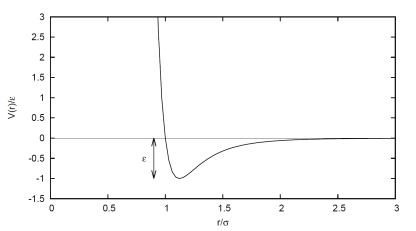
\includegraphics[width=\linewidth]{lennard_jones}
	\caption{Potencial de Lennard-Jones}
	\label{figure_lennard}
\end{figure}

\subsection{Metrópolis Monte Carlo}

Las simulaciones por ordenador juegan un papel muy importante en muchos campos de la física como la mecánica estadística. La razón de su importancia en la mecánica estadística radica en que muchos de sus modelos, incluso los que parecen más simples, son teóricamente intratables, por lo que es necesario recurrir a métodos computacionales que permiten encontrar buenas estimaciones.

De entre estos métodos, los denominados de Monte Calor han demostrado ser muy potentes. Estos consisten en algoritmos que tratan de explorar el espacio de posibles soluciones de forma aleatoria pero controlada para, a partir de su comportamiento, obtener una solución en términos estadísticos. 


Aplicaremos estos conceptos para hacer simulaciones del potencial Lennard-Jones. En particular, mediante el algortimo de Métropolis obtendremos una muestra de posibles configuraciones, las cuales tendrán una probabilidad de darse proporcional al factor de Boltzmann

\begin{equation}
	P(E) \propto e^{- \frac{E}{K_b T}}
\end{equation}